\documentclass[a4paper,12pt]{article} 
\usepackage{german}
\usepackage[T1]{fontenc}
\usepackage[utf8]{inputenc}
\usepackage{graphicx}
\usepackage{float}
\usepackage[numbib]{tocbibind}
\begin{document}
\renewcommand\refname{Referenzen und Nachweise}

\begin{titlepage}
\author{Elena Noll\\
		Sven-Hendrik Haase}
\title{Erkennung von Toren beim RoboCup} 
\date{\today} 
\maketitle
\thispagestyle{empty}
\end{titlepage}

\tableofcontents

\newpage

\section{Einführung}
Diese Arbeit beschäftigt sich mit der Bilderkennung der Tore im RoboCup.
Wichtig ist hierbei zu wissen, dass der RoboCup in verschiedenen Ligen
angeboten wird, die jeweils verschiedene Tore einsetzen. Dies wird später
genauer erläutert. Es werden zudem zwei von vielen möglichen Verfahren zur Erkennung
der Tore genauer vorgestellt.

\section{Tore im RoboCup}
Die Tore im RoboCup haben genau wie beim "normalen" Fussball mit menschlichen
Spielern die Funktion, Punkte zu werten, indem der Ball vom jeweils anderen Team über die
Torlinie geschossen wird.
Der RoboCup besteht aus verschiedenen Ligen, die grob ihrer Größe nach
gestaffelt sind. Das Tor jeder Liga kann sich jedes Jahr unabhängig von den
anderen Ligen verändern. Der allgemeine Gedanke hierbei ist, dass die
Anforderungen an die Roboter jedes Jahr wachsen sollen, indem die Schwierigkeit
inkrementell erhöht wird. Dies wird beispielsweise durch gleichfarbige Tore
bewerkstelligt, was die Selbstlokalisation der Roboter stark erschwert und die Teams herausfordert,
diese neue Hürde zu überkommen.

\subsection{Middle Size League}

\begin{figure}[H]
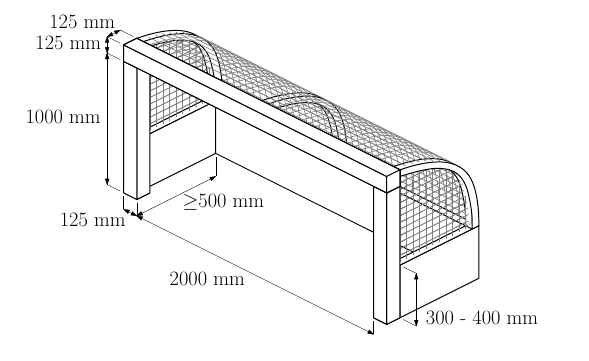
\includegraphics{middlesize-goal.png}
\caption{Tor in der Middle Size League}
\label{fig:goal-msl}
\end{figure}

Die Grafik zeigt die Maße an. Die Farbe beider Tore bei der Middle Size League ist seit einigen
Jahren weiss. Eine besondere Schwierigkeit bei der Bilderkennung stellt hierbei das ebenfalls
weisse Netz dar, welches
fälschlicherweise als Feldlinie erkannt werden könnte. Die Tore besitze eine geschlossene Form. Das
Netz ist solide und behält seine Form, was es von "echten" Netzen beim Fußball unterscheidet.


\subsection{Humanoid League}
\begin{figure}[H]
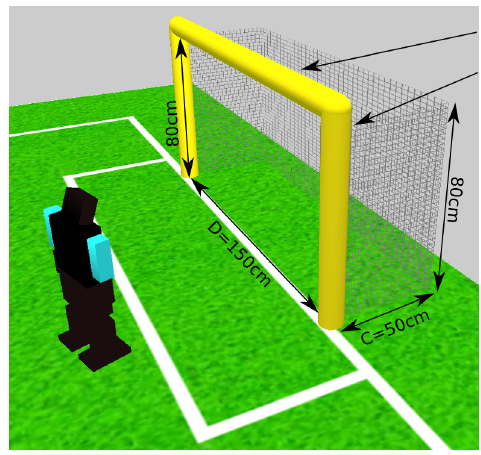
\includegraphics{humanoid-kidsize-goal.png}
\caption{Tor in der Kid Size Humanoid League}
\label{fig:goal-human-kid}
\end{figure}

\begin{figure}[H]
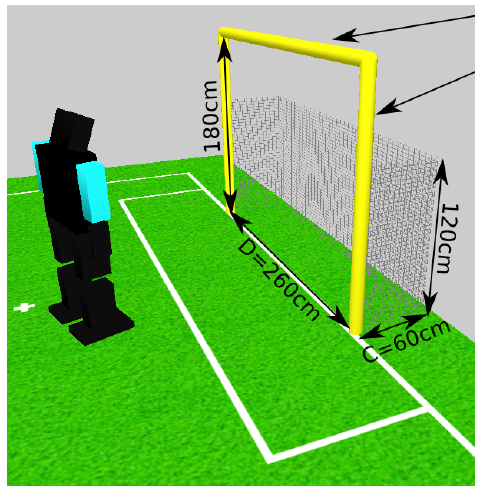
\includegraphics{humanoid-adultsize-goal.png}
\caption{Tor in der Adult Size Humanoid League}
\label{fig:goal-human-adult}
\end{figure}
Wie in den Grafiken dargestellt, gibt es für die beiden Größen der Humanoid League auch jeweils ein
passendes Tor. Anders als bei der Middle Size League sind die Torfarben jedoch unterschiedlich:
Eines ist blau, das andere ist gelb. Das Regelwerk von 2012 stellt in Aussicht, dass sich dies bald
ändern könnte. Hinter dem Tor befindet ein engmaschiges, solides Netz mit dunkler Farbe.

\subsection{Standard Platform League}
\begin{figure}[H]
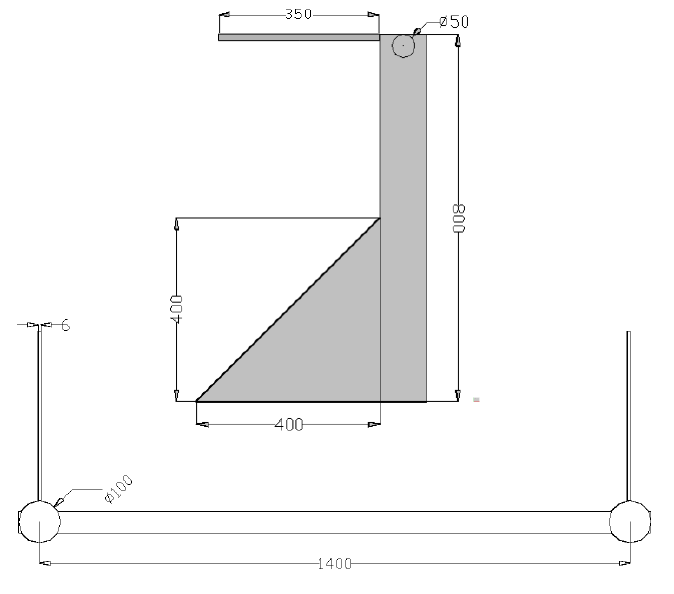
\includegraphics[scale=0.8]{spl-goal.png}
\caption{Tor in der Standard Platform League}
\label{fig:goal-spl}
\end{figure}
Bei den Toren der Standard Platform League fallen die zusätzlichen Keile an Torpfosten auf, die
sich nach hinten zur Befestigung des Netzes erstrecken. Diese Keile können zusätzlich bei der
Bildverarbeitung dazu benutzt werden, den Roboter sich lokalisieren zu lassen, da sie mehr
geometrische Informationen bieten, als ein einzelner Torpfosten. Zu bemerken ist auch, dass die
Farbe beider Tore seit 2012 auf gelb festgelegt ist.

\section{Bilderkennung}
Die optische Erkennung von Toren im RoboCup ist ein wichtiger Bestandteil des Wettbewerbs. Obwohl
Bilderkennung im Allgemeinen nichts Neues ist, ist das stetige Verbessern bestehender Verfahren und das
Finden neuer Methoden Teil fortlaufender Forschung. Die sich ständig ändernden Regeln des RoboCups
sorgen mitunter auch dafür, dass bestehende Algorithmen ihre Effektivität verlieren und jährlich
revisioniert werden müssen. In dieser Arbeit werden zwei von vielen Verfahren vorgestellt, weil die
beiden Verfahren die unterschiedlichen Herangehensweisen gut veranschaulichen.

\subsection{Probleme}
Die allgemeinen Probleme, die es bei der Bilderkennung für Tore zu lösen gilt, sind aufgrund
der Umstände mannigfaltig: Durch die Mobiltät des Roboters ändert sich die Perspektive ständig. Das
führt dazu, dass das Bild des Tores, welches der Roboter erhält, teilweise startk verzerrt wird. Es
kann beispielsweise vorkommen, dass der Roboter nur den unteren Teil eines einzigen Pfostens sieht.
Dies führt zu großen Probleme bei der Lokalisation anhand dieses Bildes alleine, sodass das der
optische Momenteindruck so nicht ausreicht, um festzustellen, wo sich der Roboter befindet. Das
optische System muss also in ein umfassenderes System eingebettet werden. Die mittlerweile teils
gleichfarbigen Tore kommen hierbei erschwerend hinzu. \\

Ein weiteres Probleme wurde bereits erwähnt: Tornetze können teilweise als Feldlinien erkannt
werden. Außerdem können Teile vom Tor verdeckt sein (z.B. von anderen Robotern) oder es könnten
Hindernisse in der Schussbahn stehen. Letzteres ist nicht direkt ein Problem der Torerkennung, aber
es ist damit eng verwandt, denn ein Torschussversuch kann nur erfolgreich sein, wenn der Schuss
nicht vorher blockiert wird. Der Roboter muss sich also bewusst sein, wie er sich positionieren
muss, damit ein Schussversuch gelingen kann.

\subsection{Erkennung mittels geometrischer Relationen}
Bei diesem Verfahren, das die geometrischen Sturkturen der Elemente im RoboCup ausnutzt, werden
vier Schritte ausgeführt:
\begin{enumerate}
	\item Farbkalibrierung im YUV-Farbraum
	\item Farbsegmentierung
	\item Erkennung des Horizonts
	\item Extraktion der Torpfosten und Modellierung
\end{enumerate}

\subsubsection{Farbkalibrierung YUV-Farbraum}
\begin{figure}[H]
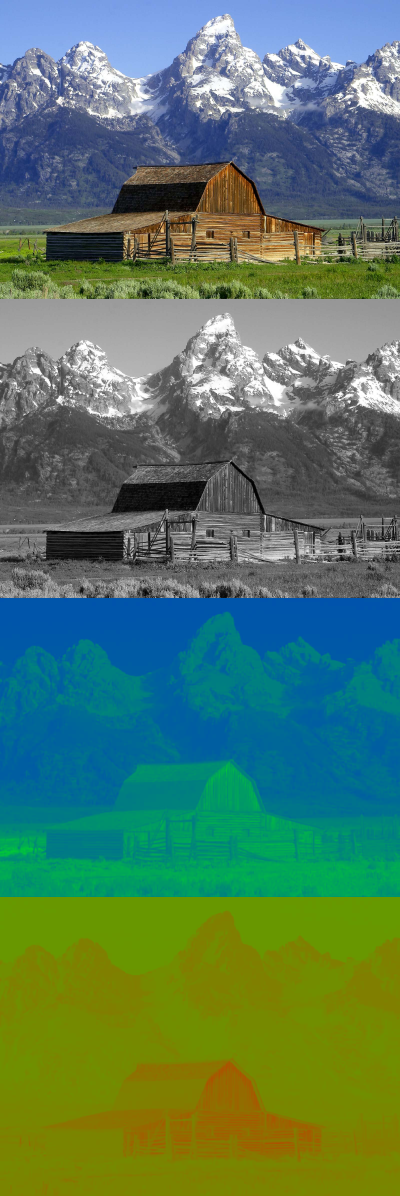
\includegraphics[scale=0.5]{Barn-yuv.png}
\caption{Beispiel eines Bildes im YUV-Farbraum}
\label{fig:yuv}
\end{figure}

\subsubsection{Farbsegmentierung}

\begin{figure}[H]
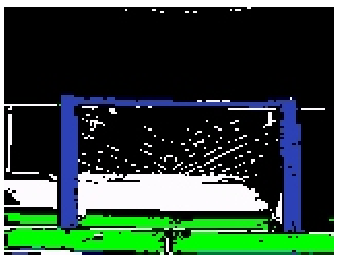
\includegraphics{segmented-view2.png}
\caption{Farbsegementiertes Bild}
\label{fig:color-seg}
\end{figure}

\begin{figure}[H]
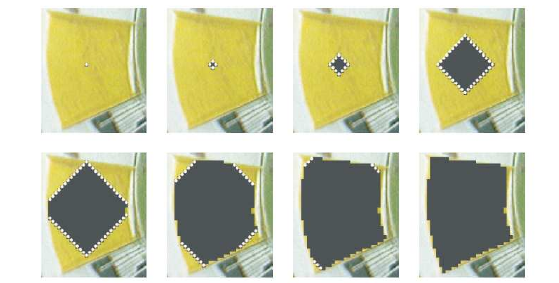
\includegraphics[scale=0.9]{region-growing.png}
\caption{Vorgang der Farbsegmentierungs-Algorithmus}
\label{fig:color-seg-algo}
\end{figure}

\begin{figure}[H]
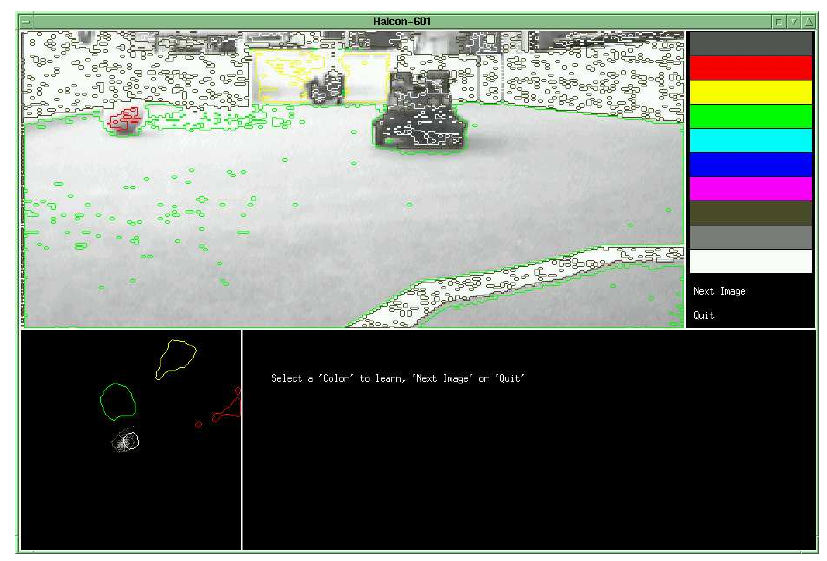
\includegraphics[scale=0.6]{training-tool.png}
\caption{Programm zur interaktiven Echtzeit-Farbsegmentierung}
\label{fig:color-seg-tool}
\end{figure}

\begin{figure}[H]
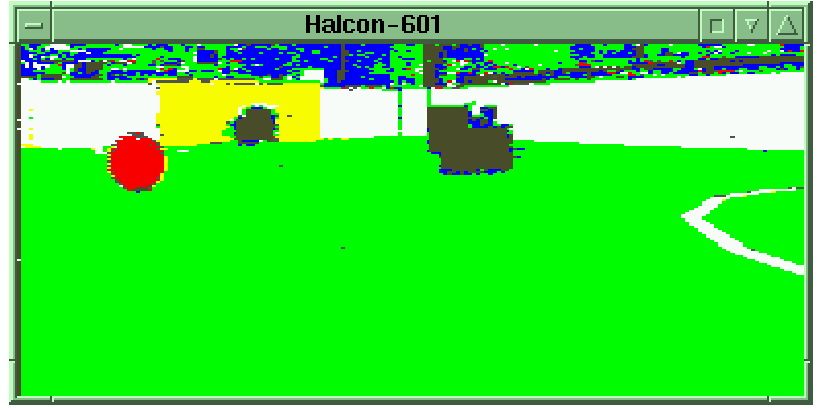
\includegraphics[scale=0.6]{segmented-view.png}
\caption{Segmentiertes Kamerabild}
\label{fig:color-seg-cam}
\end{figure}

\subsubsection{Erkennung des Horizons}
\begin{figure}[H]
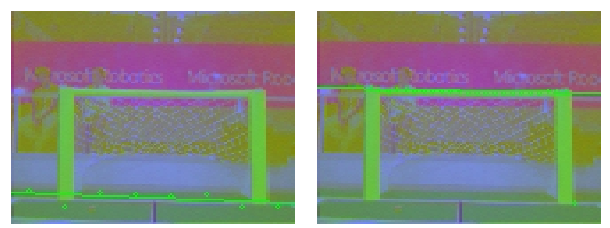
\includegraphics[scale=0.8]{geometric-plane.png}
\caption{Geometrische Horizonterkennung}
\label{fig:geom-horiz}
\end{figure}

\subsubsection{Extraktion der Torpfosten und Modellierung}
\begin{figure}[H]
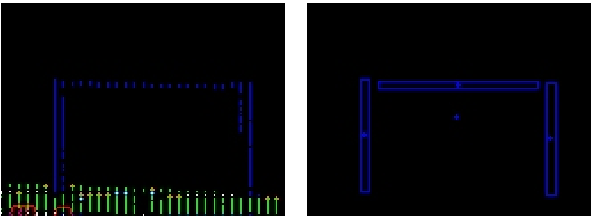
\includegraphics[scale=0.8]{goal-blobs.png}
\caption{Links: Extraktion; Rechts: Modellierung}
\label{fig:model}
\end{figure}

\subsubsection{Beispiele}
\begin{figure}[H]
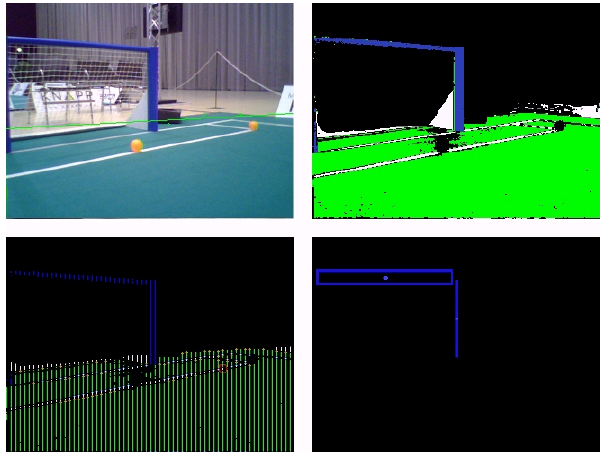
\includegraphics[scale=0.8]{example-detection1.png}
\caption{Beispiel 1 des Verfahrens}
\label{fig:example1}
\end{figure}

\begin{figure}[H]
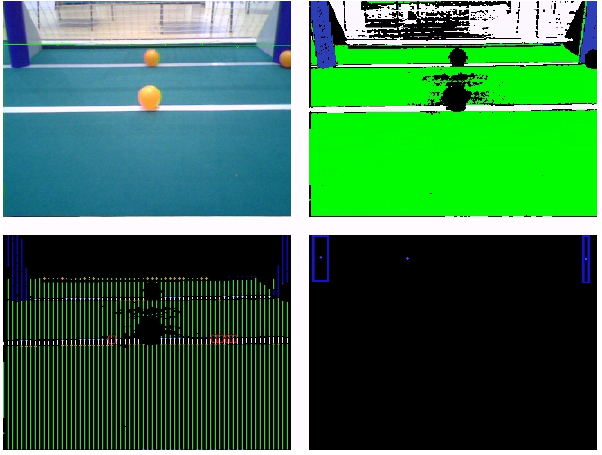
\includegraphics[scale=0.8]{example-detection2.png}
\caption{Beispiel 2 des Verfahrens}
\label{fig:example2}
\end{figure}

\begin{figure}[H]
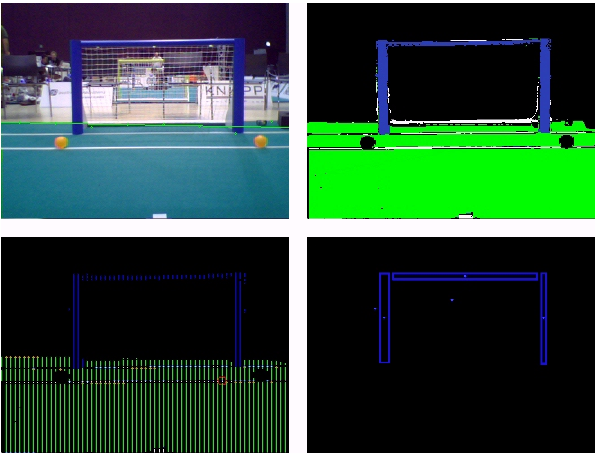
\includegraphics[scale=0.8]{example-detection3.png}
\caption{Beispiel 3 des Verfahrens}
\label{fig:example3}
\end{figure}

\begin{figure}[H]
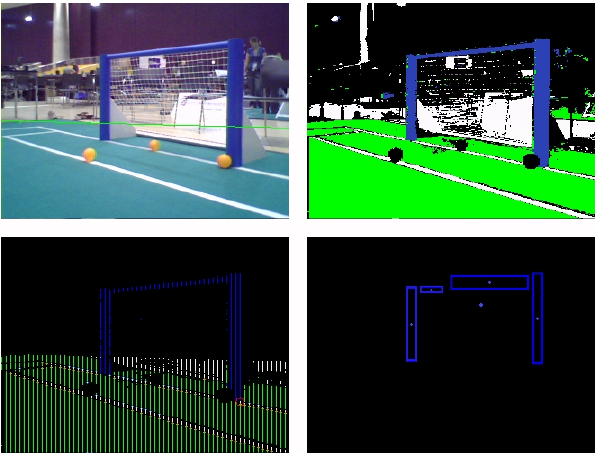
\includegraphics[scale=0.8]{example-detection4.png}
\caption{Beispiel 3 des Verfahrens}
\label{fig:example4}
\end{figure}

\subsection{Erkennung mittels Hough-Transformation}
\subsubsection{Farbfilterung im HSV-Farmraum}
\subsubsection{Zielsetzung der Hough-Transformation}
\subsubsection{Beispiel}
\subsubsection{Eigenschaften der Hough-Transformation}

\section{Fazit}

\bibliography{general}
\begin{thebibliography}{9}

\bibitem{lamport94}
  Leslie Lamport,
  \emph{\LaTeX: A Document Preparation System}.
  Addison Wesley, Massachusetts,
  2nd Edition,
  1994.

\end{thebibliography}

\listoffigures

\end{document}
